\documentclass{llncs} 
\usepackage{url} 
\usepackage{times}
%For math symbols like number classes
\usepackage{amsfonts}
\usepackage{amssymb}
\usepackage{amsmath}
%\usepackage{amsthm}
\usepackage{floatflt}
\usepackage{wrapfig}
\usepackage{multirow}

\usepackage{graphicx}
\usepackage{graphics}

\usepackage[boxed,linesnumbered,vlined,slide]{algorithm2eCustom}

%\usepackage[numbers,sort&compress]{natbib}

\usepackage{color}

\newcommand{\ffh}[1]{\textbf{TODO: \textit{#1}}} 

\newcommand{\mdns}{\ac{MD}}
\newcommand{\md}{\mdns \xspace}
\newcommand{\mdsns}{{\mdns}'s}
\newcommand{\mds}{\mdsns \xspace}

\newcommand{\ls}{\lsns \xspace}
\newcommand{\lsns}{LS}
\newcommand{\lss}{\lssns \xspace}
\newcommand{\lssns}{LSs}

\newcommand{\spathns}{\ac{SP}}
\newcommand{\spath}{\spathns \xspace}
\newcommand{\spathsns}{{\spathns}s}
\newcommand{\spaths}{\spathsns \xspace}

\newcommand{\oscns}{\ac{OSC}}
\newcommand{\osc}{\oscns \xspace}

\newcommand{\lruns}{\ac{LRU}}
\newcommand{\lru}{\lruns \xspace}
\newcommand{\lrusns}{{\lruns}s}
\newcommand{\lrus}{\lrusns \xspace}

\newcommand{\fifons}{\ac{FIFO}}
\newcommand{\fifo}{\fifons \xspace}

\newcommand{\spsns}{\ac{SPS}}
\newcommand{\sps}{\spsns \xspace}

\newcommand{\salgons}{$\mathsf{PScache}$}
\newcommand{\salgo}{\salgons \xspace}

\newcommand{\poins}{\ac{POI}}
\newcommand{\poi}{\poins \xspace}
\newcommand{\poisns}{{\poins}'s}
\newcommand{\pois}{\poisns \xspace}

\newcommand{\naive}{\naivens \xspace}
\newcommand{\fair}{\fairns \xspace}
\newcommand{\naivens}{\textbf{Naive}}
\newcommand{\fairns}{\textbf{Fair}}

\newcommand{\zebox}[1]{$|\underline{\overline{#1}}|$}

\newcommand{\lpar}{(}
\newcommand{\rpar}{)}

\SetKwBlockLRS{JRBegin}
\newcommand{\funcc}[3]{\emph{\textbf{#1}}\ensuremath{\lpar #2 \rpar} \JRBegin{#3}}
%\newcommand{\func}[2]{\emph{\textbf{#1}}\ensuremath{\lpar #2 \rpar} \\}


%To change extension of algorithm2e use \algoext{A}, \algoext{B}, \Algoext{}
\newcommand{\algoext}[1]{\renewcommand{\thealgoext}{#1}}

%------------------------------------------------------------------------- 
% take the % away on next line to produce the final camera-ready version 
\pagestyle{plain}
%
%------------------------------------------------------------------------- 
\begin{document}

\newtheorem{thm}{Theorem}[section]
\newtheorem{cor}[thm]{Corollary}
\newtheorem{lem}[thm]{Lemma}

\SetKwBlockLRS{LRSBegin}


\title{A Location Privacy Aware Friend Locator}
\toctitle{A Location Privacy Aware Friend Locator}
\titlerunning{A Location Privacy Aware Friend Locator}

\author{Laurynas \v{S}ik\v{s}nys
\and Jeppe R. Thomsen
}
\institute{Aalborg University\\ Department of Computer Science \\ Selma Lagerl\o fs Vej 300, DK-9220 Aalborg \O \\ Denmark}
\maketitle

\begin{abstract}
 % All the papers either solve the problem of a more efficient cache in a specific domain, or use the network domain,  which are both relevant, but not really useful when looking at shortest path caching.
% 
% The papers show some interesting ways to use cache, but ultimately their approaches are very domain or query specific so their approaches to caching and cache replacement/invalidation can not be applied directly.


abstract...

Lorem ipsum dolor sit amet, consectetur adipiscing elit. Nunc luctus mattis pretium. Mauris egestas risus non lectus dapibus condimentum. Vestibulum at lacus sit amet elit rutrum venenatis sit amet sed turpis. Nam ullamcorper, urna aliquet venenatis tempor, dolor enim egestas neque, ac feugiat felis neque et libero. Vivamus in augue urna. Integer euismod interdum felis, a porta quam posuere at. Duis molestie leo ullamcorper mauris sodales porta. Praesent cursus, tortor a iaculis blandit, mauris tellus suscipit nibh, in condimentum elit eros nec mauris. In hac habitasse platea dictumst.

Phasellus eget tortor eget diam dignissim pretium nec ut nibh. Morbi bibendum nibh et eros tristique rhoncus. Suspendisse dolor erat, lacinia ut ullamcorper vitae, dictum nec dolor. Etiam egestas tempus fermentum. Donec commodo feugiat lorem. Donec facilisis pharetra leo, sit amet cursus turpis convallis eu. Sed fermentum sapien quam, quis porttitor est.
\end{abstract}
\section{Multi-weight} \label{sec:intro}


\begin{table}
\begin{tabular*}{\columnwidth}{|l|p{0.76\columnwidth}|}
\hline
\bf Symbol		& \bf Meaning \\\hline
$G\mathbf{(V,E)}$ 	& A graph with node set $V$ and edge set $E$ \\\hline 
$v_i$			& A node in $V$ \\\hline 
$(v_i,v_j)$		& An edge in $E$ \\\hline 
$\omega_k(v_i,v_j)$	& The edge weight of $(v_i,v_j)$ using weight category $\varsigma_k \in \mathcal{W}$ \\\hline
$\mathcal{W}$		& Set of possible weight categories $\mathcal{W}$, where $\varsigma_k$ denotes the category $k$ \\\hline

$Q_{s,t,w}$		& \spath query from node $v_s$ to node $v_t$, using weight $w$\\\hline
$P_{s,t,w}$		& The \spath result of $Q_{s,t,w}$ \\\hline
$|P_{s,t,w}|$		& The size of $P_{s,t,w}$ (in number of nodes) \\\hline
$E_{s,t,w}$		& The expense of executing query $Q_{s,t,w}$ \\\hline
$\chi_{s,t,w}$		& The frequency of a \spath with weight type w \\\hline
$\Psi$ 			& The Cache \\\hline
$\mathfrak{U}^w(P_{s,t,w})$& The set of all subpaths in $P_{s,t,w}$ \\\hline
$\mathfrak{U}^w(\Psi)$	& The set of all subpaths of paths in $\Psi$ \\\hline
$\gamma^w(\Psi)$		& The total benefit of the content in the cache \\\hline

$d_{s,t,w}$		& The \spath distance of a path $P_{s,t,w}$ \\\hline
$\mathcal{QL}^w$		& Query log of search queries \\\hline
\end{tabular*}
\caption{Table of Symbols \textbf{MW}}
\label{tab:symbols}
\end{table}

% 
% 
% \begin{algorithm}[bht]
% \dontprintsemicolon
% \SetVline
% 
% \SetKwInOut{Input}{input}\SetKwInOut{Output}{output}\SetKw{Return}{return}
% 
% \Input{
% 
% 	$(q,R)$: A Range query\;
% 	$\mathcal{O}$: A set of POI \;
% }
% 
% \Output{
% 
% 	A set \poi $\in \mathcal{O}$ \;
% }
% 
% \funcc{Fair}{(q,R), \mathcal{O}}
% {
%     \ForEach{$o_i \in \mathcal{O} : \mathfrak{d}_{q,o_i} \leq R$}
%     {
%       $candidate_{\mathcal{O}} \leftarrow o_i$ \;
%     }
%     result $\leftarrow$ \naivens((q,R), $candidate_{\mathcal{O}}$) \;
% 
%     \Return{result} \;
% }
% 
% \caption{Fair Algorithm}
% \label{alg:fair}
% \end{algorithm}


In multi-weight road networks\cite{icdeMouratidisLY10} a shortest path query may be submitted to a service provider based on different shortest path metrics or categories. A category could be the fastest route, the fewest number of edges to traverse, or of cause the actual shortest distance. These kind of queries require the \spath service provider to have several weights defined for each edge, a fair assumption on most service providers (TODO: CITE).
Such queries present a challenge to effectively cache, as the same \spath $P_{s,t,w}$ may not be valid for all weights/metrics $w$.
Two queries with identical start- and end-point can return two different \spathsns, depending on what weight category is issued with the query. Figure \ref{fig:map1} shows a map with two weight categories on each edge, $w_1,w_2$. The two queries $Q_{1,6,w_1}$ \& $Q_{1,6,w_2}$ are identical, except for the weight category. $\psi_1$ and $\psi_2$ in table \ref{tab:expsi} show the \spath result of the two queries in column "cache item". It is clear that the result of the two queries are very different because of the difference in weight category used for each result.




\begin{definition}
Let $G(V, E)$ be a graph with a set $V$ of nodes and a set $E$ of edges.
Each node $v_i \in V$ models a road junction. Each edge $(v_i, v_j) \in
E$ models a road segment. The weight or 'length' of an edge is denoted as $W(v_i, v_j, w)$, where $w \in \mathcal{W}$ is the weight type (length, travel time, scenic value, ect.).
\end{definition}



\begin{definition}{Multi-weight Search}\\
A Multi-weight Search query, denoted by $Q_{s,t,w}$ consist of a source and target vertex $s$ and $t$, plus a category $w \in \mathcal{W}$ 
The result of $Q_{s,t,w}$, denoted $P_{s,t,w}$, is a collection of connected vertices $v_s,\dotsc,v_t$ such that they form a \spath on graph $G\mathbf{(V,E)}$ using category $w \in \mathcal{W}$.
\end{definition}


Using the map1 (fig. \ref{fig:map1}) a multi-weight search query, $Q_{1,2,w}$, can be executed for two different weights, $w_1$ or $w_2$, possibly resulting in two different paths for the same start-/end-nodes, depending on the weight chosen. Table \ref{tab:expsi} shows the \spath $\psi_1$ and $\psi_2$ resulting from the same start-/end-node, but using different weights ($w_1, w_2$).


\begin{figure}[hbt]
  \center
        \includegraphics[width=0.4\textwidth]{figures/map1}
        \caption{Map1. Has a set of two weights on each edge, $w_1,w_2$.}
  \label{fig:map1}
\end{figure}

\begin{table}
\begin{tabular}{l|l|l}\hline
$\psi$		& Cache item 			& Category \\\hline  \hline
$\psi_1:$	& $\{v_1,v_3,v_4,v_5,v_6\}$ 	& ($w_1$)\\\hline
$\psi_2:$	& $\{v_1,v_3,v_6\}$ 		& ($w_2$)\\\hline
$\psi_3:$	& $\{v_1,v_3,v_4,v_5\}$ 	& ($w_1,w_2$)\\\hline
\end{tabular}
\caption{Cache items using queries $Q_{1,6,X}, Q_{1,5,X}$ with $X:\{w_1,w_2\}$, covering both weights on the map (fig \ref{fig:map1})}
\label{tab:expsi}
\end{table}


\begin{definition}{Multi-weight Query Log ($\mathcal{QL}^{w}$)}\\
A multi-weight search query log $\mathcal{QL}^w$ is a collection of time stamped queries that have been issued by users in the past.
A query is on the form $(s,t,w)$, where $s$ and $t$ is the start- and end-point respectively. $w$ is the category to be used when calculating the SP. The full form of the log, $\mathcal{QL}^{w}$,  is then: $\{(s_0,t_0,w_0),\dots,(s_i,t_i,w_i)\}$.
\end{definition}



\subsection{Cache Structure}

Paths are stored as sets of vertices $\{(s_0,t_0),\dots,(s_i,t_i)\}$ with an associated category $w \in W$ in the cache. Instead of using a single inverted list to look up whether the cache can answer a query, we use a collection of inverted lists to keep track of which $Q_{s,t,w}$ can be answered by the cache ($\Psi$), for each category in $\mathcal{W}$.
Even if a full path can only answer a query for a single weight type, then by using this approach then any sub-path able to answer for more than one weight-type will still be utilized. 

The map in figure \ref{fig:map1} depicts a simple road system with 2 different weights on each edge. The first edge weight captures edge length, while the second weight captures the of number of edges traversed, which is why each edge always contributes 1.

To answer a query $Q_{s,t,w}$ on the cache in table \ref{tab:expsi}, for each item $\psi_i$, we first check whether $w$ matches any of the entries in the category column. If $w$ matches an entry we then we check whether $s \in \psi_i$ and $t \in \psi_i$, if yes, then $\psi_i$ can answer $Q_{s,t,w}$. We search each entry in the table until either we find an match, or all entries have been examined.

If we want to answer the query $Q_{1,4,w_2}$ we will first check the category column of $\psi_1$, as it does not include $w_2$ we know it can not answer our query and we proceed to check $\psi_2$. Since $\psi_2$ can answer some query with category $w_2$ we check whether $v_1 \in \psi_2$ and $v_4 \in \psi_2$. Since $v_4 \not \in \psi_2$ we proceed to check $\psi_3$. As the category of $\psi_3$ contains $w_2$ and $v_1, v_4 \in \psi_3$ we know that $\psi_3$ can answer $Q_{1,4,w_2}$.

As the cache in table grows larger it becomes inefficient to search, so we extend the idea of using inverted list from \cite{thomsen2012}(sec. 4.2). Assuming the following four historical queries, \\
$Q_{1,6,w_1},Q_{1,6,w_2}, Q_{1,5,w_1},Q_{1,5,w_2}$ from $\mathcal{QL}^{w}$, we will have the cache items in table \ref{tab:expsi}. Using this we build a inverted list for each weight in order to quickly answer queries (see fig. \ref{fig:wilist}). 
To answer a query $Q_{v_s,v_t,w}$ we use $w$ to first find the relevant inverted list. Afterwards we do 2 look-ups in the inverted list, for $v_s$ \& $v_t$ respectively, and then check the intersection of the cache items. If the answer is non-empty there is a \spath for $Q_{v_s,v_t,w}$ in the cache. 
A more efficient approach would be to combine all the tables together and make the key (weight,vertex). This would reduce the number required lookups to two, and since the tables most likely will have some identical items, then we may also have a chance to optimize the number of entries.

\begin{figure}[hbt]
  \center
        \includegraphics[width=0.20\textwidth]{figures/wilist}
        \caption{Cache structure for inverted lists using map1 (fig. \ref{fig:map1}) and cache elements from table \ref{tab:expsi}}
  \label{fig:wilist}
\end{figure}

\subsection{Benefit Model}

We extend the benefit driven benefit model introduced in \cite{thomsen2012}. We introduce what changes are needed to capture the benefit of \spaths with \textit{multi-weight search}.
Equation \ref{eq:phiw}, \ref{eq:benefitw}, \ref{eq:upsw}, and \ref{eq:cachebenefitw} define the existing functions with restriction on $w$.


We have to answer two important questions:
\begin{enumerate}
\item \label{quest:impone} Which queries $Q_{s,t,w}$ can be answered by the path $P_{s,t,w}$?
\item \label{quest:imptwo} For query $Q_{s,t,w}$ what is the benefit if added to the cache.
\end{enumerate}

Question \ref{quest:impone} can be answered by the updated lemma \ref{lem:weightedoptimalproperty} (from \cite{thomsen2012}). A path $P_{a,b,d}$ contains the path $P_{s,t,w}$ if they share the same weight and both $v_s$ \& $v_t$ are on $P_{a,b,d}$. With this we get the updated definition for the \textit{answerable query set}, $\mathfrak{U}^w(P_{a,b,d})$, for path $P_{a,b,d}$:

\begin{equation} \label{eq:phiw}
\mathfrak{U}^w(P_{a,b,d}) = \{ P_{s,t,w} : s, t \in P_{a,b,d},  s \neq t,  d = w\}
\end{equation}

Equation \ref{eq:phiw} finds all sub-paths of SP $sp$ with weight category $w$. Using cache item $\psi_1$ from $Q_{v_1,v_6}$ in table \ref{tab:expsi}, the answerable queryset is: $\mathfrak{U}^w(P_{1,6,w_1}) = \{P_{1,3,w_1},P_{1,4,w_1},P_{1,5,w_1},P_{1,6,w_1},P_{3,4,w_1},$ $P_{3,5,w_1},P_{3,6,w_1},P_{4,5,w_1},P_{4,6,w_1},P_{5,6,w_1}\}$ 


In regards to question \ref{quest:imptwo} we update the \textit{benefit} equation $\gamma(\Psi)$ to consider weight categories:

\begin{equation} \label{eq:benefitw}
\gamma^w(P_{a,b,d}) = \sum\limits_{P_{s,t,w} \in \mathfrak{U}^w(P_{a,b,d})} \chi_{s,t,w} \bullet E_{s,t,w}
\end{equation}

Equation \ref{eq:benefitw} defines $benefit$ and makes it clear how much can we expect to save, in total, if path $P_{a,b,d}$ is in the cache. It is calculated based on the historical statistics defined by $\chi_{a,b,d}$ (equation \ref{eq:chiw}) and the cost of calculating the \spathns, $E_{a,b,d}$.


\begin{equation} \label{eq:chiw}
\chi_{s,t,w} =  |\{ Q_{b,e,w} \in \mathcal{QL}^{w}: s, t \in Q_{b,e,w} \}|
\end{equation}

\begin{equation} \label{eq:chiSingleToRegw}
 \hat{\chi}_{R_i, R_j, w} = \sum\limits_{v_s \in R_i} \sum\limits_{v_t \in R_j} \chi_{s,t,w}
\end{equation}


\begin{equation} \label{eq:chiregw}
\chi_{s,t,w} = \frac{ \hat{\chi}_{R_i, R_j, w} }{|R_i| \cdot |R_j|}
\end{equation}



Based on how often we have seen the path, and its subpaths, in the query log $\mathcal{QL}^{w}$, equation \ref{eq:chiw} defines the benefit of a path, for a single path. Equation \ref{eq:chiSingleToRegw} for $\hat{\chi}_{R_i, R_j, w}$ sums up all $\chi_{s,t,w}$ going from a vertex $v_s$ in region $R_i$ to a vertex $v_t$ in $R_j$. Using equation \ref{eq:chiSingleToRegw} we can then define $\chi_{s,t,w}$ for regions as equation \ref{eq:chiregw}.




\begin{lemma} \label{lem:weightedoptimalproperty}
\textbf{Weighted optimal subpath property} (modified from \cite{thomsen2012}, Lemma 1)\\

The \spath $P_{a,b,d}$ contain the \spath $P_{s,t,w}$ if $v_s \in P_{a,b,d}, v_t \in {P_a,b,d}$ and $d = w$, where $d,w \in \mathcal{W}$
Let $P_{a,b,d}$
Specifically, let $P_{a,b,d} = \langle v_{x_0},v_{x_1},v_{x_2},...,v_{x_m}\rangle$. 
We have $P_{s,t,w} = \langle v_{x_i},v_{x_i+1},...,v_{x_j}\rangle$ if $v_s = v_{x_i}, v_t = v_{x_j}$, and $w = d$ for some i,j such that $0 \leq i \leq j \leq m$
\end{lemma}



For the general case where the cache contains more than one path, the updated equations are shown below:

\begin{equation} \label{eq:upsw}
 \mathfrak{U}^w(\Psi) = \bigcup\limits_{P_{a,b,w} \in \Psi} \mathfrak{U}^w(P_{a,b,d})
\end{equation}

Equation \ref{eq:upsw} finds the set of unique paths with weight $w$ from $\Psi$, which is either a path from $a$ to $b$, or a sub-path of such a path. This is the answerable set of paths using  $P_{a,b,d}$.

\begin{equation} \label{eq:cachebenefitw}
\gamma^w(\Psi) = \sum\limits_{P_{s,t,w} \in \mathfrak{U}^w(\Psi)} \chi_{s,t,w} \cdot E_{s,t,w}
\end{equation}

Equation \ref{eq:cachebenefitw} calculate the benefit of the cache with respect to a specific weight category, using $\chi_{s,t,w}$ and $E_{s,t,w}$, in the same way $\chi_{s,t}$ is calculated using $\chi_{s,t}$ and $E_{s,t}$.





The same query with different weight can result in different cache items. In table \ref{tab:expsi} the queries $Q_{1,6,w_1},Q_{1,6,w_2} \in \mathcal{QL}^{w}$, the two only differing on the weight parameter. The two queries results in both $\psi_1$ and $\psi_2$ being in the cache, since the query returns two different paths for weights $w_1$ and $w_2$. 
It can of cause also be the case that no matter what weight we use, the \spath is the same. The queries $Q_{1,5,w_1},Q_{1,5,w_2} \in \mathcal{QL}^{w}$ are an example of this, as the \spath does not change for $w_1$ or $w_2$. 
An important aspect to notice is that though a complete cache item may only valid for a single weight category, then a sub path of the \spath can be valid for several categories. This can e.g. be seen in $\psi_1$ (table \ref{tab:expsi}) where the path is only valid for $w_1$, but $\psi_1 \setminus v_6$ is identical to $\psi_3$ which we already know is valid for both $w_1,w_2$. Avoiding this duplication of information could e.g. be done by using inverted lists as in fig. \ref{fig:wilist} to store the information on weight category. If we do so we will not need to store $\psi_3$, since $\psi_3 \in \psi_1$.





% 
% \begin{tabular}{|l|l|}\hline
% \textbf{V} &	\textbf{Cache Item} \\\hline
% $V_1$	&	$\psi_1, \psi_3$ \\\hline
% $V_3$	&	$\psi_1, \psi_3$ \\\hline
% $V_4$	&	$\psi_1, \psi_3$ \\\hline
% $V_5$	&	$\psi_1, \psi_3$ \\\hline
% $V_6$	&	$\psi_1$ \\\hline
% \end{tabular}
% \vspace{2em}
% 
% \begin{tabular}{|l|l|}\hline
% \textbf{V} &	\textbf{Cache Item} \\\hline
% $V_1$	&	$\psi_2, \psi_3$ \\\hline
% $V_3$	&	$\psi_2, \psi_3$ \\\hline
% $V_4$	&	$\psi_3$ \\\hline
% $V_5$	&	$\psi_3$ \\\hline
% $V_6$	&	$\psi_2$ \\\hline
% \end{tabular}

\section{Direction Assistance}


\begin{table}
\begin{tabular*}{\columnwidth}{|l|p{0.76\columnwidth}|}
\hline
\bf Symbol		& \bf Meaning \\\hline
$G\mathbf{(V,E)}$ 	& A graph with node set $V$ and edge set $E$ \\\hline 
$v_i$			& A node in $V$ \\\hline 
$(v_i,v_j)$		& An edge in $E$ \\\hline 

$Q_{s,t}$		& \spath query from node $v_s$ to node $v_t$, using \textit{path level l}\\\hline
$P_{s,t}$		& The \spath result of $Q_{s,t,l}$, using \textit{path level l}. \\\hline
$|P_{s,t}|$		& The size of $P_{s,t,l}$ (in number of nodes) \\\hline
$E_{s,t,l}$		& The expense of executing query $Q_{s,t,l}$ \\\hline
$\chi_{s,t,l}$		& The frequency of a \spath with level $l$ \\\hline
$\Psi$ 			& The Cache \\\hline
$\mathfrak{U}_l(P_{s,t,l})$& The set of all subpaths in $P_{s,t,l}$ \\\hline
$\mathfrak{U}_l(\Psi)$	& The set of all subpaths of paths in $\Psi$ \\\hline
$\gamma_l(\Psi)$	& The total benefit of the content in the cache \\\hline

$d_{s,t,l}$		& The \spath distance of a path $P_{s,t,l}$ \\\hline

$\mathcal{QL}$		& Query log of search queries (see \cite{thomsen2012}) \\\hline
\end{tabular*}
\caption{Table of Symbols \textbf{DA}}
\label{tab:symbols}
\end{table}

When looking for directions to some place, a user who issues a \spath query does not actually care about the full \spathns\cite{sigmodTaoSP11}, but rather the user just wants to know when a new action is needed (turn left, right, or any action other action, besides following the current path. This is what GPS devices usually do. GPS devices usually only alerts the user if an action is needed, otherwise the user should just continue on the current path.


The same query can be saved at many different levels of detail, figure \ref{fig:minroute} shows a route from S to T, where each node on the route is marked as belonging to the $fine$\textbf{(F)} or $coarse$\textbf{(C)} level of detail (difference explained later). Table \ref{tab:psilvlcontent}, $\psi_1$, shows the set of nodes included in a \spath depending on the level of detail desired. 


There are 2 overall $levels$ that directions to follow a \spath can be given:

\begin{tabular}{@{}l@{  } p{21em} }
Fine ({\bf F})		& The directions are given for every single node on the \spathns, regardless of whether there are any option to change directions. \\
Coarse ({\bf C})	& The directions are given only when it is necessary to change directions, i.e. it does not matter how many side roads are passed, as long as the instruction is ostensibly "continue straight", then the instruction will not be included. Only if it is really necessary to make an action, such as turning, will the node be included in the instructions.
\end{tabular}

Both $fine$ and $coarse$ will always include the start- and end-node. An alternative (\textbf{A}) middleway could be to have the directions be given only for nodes where it is possible to change direction/turn and we will be using this alternative in figure \ref{tab:psilvlcontent} and \ref{tab:directioninvlists}, however any alternative $(\textbf{A}):(\textbf{C}) \subseteq (\textbf{A}) \subseteq (\textbf{F})$ is possible. 

When using (\textbf{F}) the advantage is that all subpaths of a \spath in the cache will be answerable, this scheme may however take op a lot of space for subpaths that are never seen, and therefor contribute no benefit to the cache.

Using (\textbf{C}) the advantage is that, especially on longer \spathsns, it will consume less space, while still maintaining enough information in the cache, enabeling it to answer some sub-queries, assuming the result includes some actions. The downside is of cause that the reduced number of vertices stored also negatively impacts the number of queries that can be answered by the \spath when it is in the cache.

It may be desireble to use some alternative (\textbf{A}) to gain the benefit of being able to answer more paths than a cache item found with (\textbf{C}) allows for, and at the same time not have to store any nodes that we do not consider useful (according to equation \ref{eq:benefitl} and \ref{eq:cachebenefitl}).


In figure \ref{fig:minroute} a path from S to T is shown. Each vertex is labeled based on what level of directions each node would be included in, according to the enumeration of (\textbf{F}) and (\textbf{C}) above. Alternative \textbf{A}) is not shown on the map.


\begin{figure}[hbt]
  \center
        \includegraphics[width=0.4\textwidth]{figures/minroute}
        \caption{$Q_{1,11}$: Bold line from S to T denote travel route. $l$=(\textbf{F}): All nodes on the path has an (F), forming the complete path. 
        $l$=(\textbf{C}): Circles with a (C) denote the minimum set of nodes needed to navigate from S to T}
  \label{fig:minroute}
\end{figure}


\begin{definition}\label{def:direction} {Direction}\\
The \textit{directions} of a query $Q_{s,t}$, where the detail level $l$ is specified by 1:(\textbf{F}), 100:(\textbf{C}), and some an Alternative(\textbf{A}):(\textbf{C}) $\leq$ (\textbf{A}) $\leq$ (\textbf{F}) , are a set of vertex neighbour pairs $\{(v_i,v_j),...\}$, each pair consisting of two connected nodes on $P_{s,t}$, representing a instruction at a node $v_i$, to take the path towards node $v_j$, where$v_i,v_j \in V$ on the \spath $P_{s,t}$.
$l$ is a system parameter set by the service provider.
\end{definition}

Figure \ref{fig:minroute} illustrates the $directions$ on query $Q_{1,11}$ for $l$ being set to both (\textbf{C}) and (\textbf{F}). For l=(\textbf{F}) the $directions$ include the all vertices on the bold path from S to T. For l=(\textbf{C}) the $directions$ only include the circled vertices: The start- and end-vertex plus a pair of neighbouring nodes each time the default action of going straight needs to be changed because the path turns where there are more than one choice.

\begin{definition}
Let $G(V, E)$ be a graph with a set $V$ of nodes and a set $E$ of edges.
Each node $v_i \in V$ models a road junction. Each edge $(v_i, v_j) \in
E$ models a road segment. The weight (length) of an edge is denoted as $W(v_i, v_j)$.
\end{definition}


\begin{definition}{\spathns: Query and Result}\\
A shortest path query, denoted by $Q_{s,t}$ consist of a source and target node, $v_s,v_t$.

The result of $Q_{s,t}$, denoted $P_{s,t}$, is a collection of nodes on the \spath from $v_s$ to $v_t$ (on the graph G) with each node associated with a direction (definition \ref{def:direction}).
We can represent $P_{s,t}$ as a list of pairs (node, neighbour node): $\langle (v_{s},v_{x_{}}), (v_{x_1},v_{x_{1n}}), \dots ,(v_{x_n},v_{x_{nn}}) \rangle$, where each pair contains a set of neighbouring vertices from $G$.
\end{definition}




\subsection{Cache Structure}

Cache items can be stored just as they did before \cite{thomsen2012}, either in a path array or as a graph representation. 

Table \ref{tab:directioninvlists} shows the inverted lists for different detail levels, based the cache content in table \ref{tab:psilvlcontent} and the map from figure \ref{fig:minroute}. Table \ref{tab:directioninvlists} shows the tables as three separate tables, there is however no reason they could not be combined, so different keys, $v_i$, point to the same data.

Figuring out at what detail level paths should be stored in the cache, and whether the should be stored in a path array or as a graph representation is one of the interesting questions we want to answer. 

For longer \spaths that are relatively simple, meaning few instructions are needed, we will store very few nodes at level (\textbf{C}). This could be a problem as we have no information about how to traverse large parts of such a shortest path, even if such parts may be have high benefit (high $chi$ values for pairs of nodes on the path). We could possibly use the $\chi$ benefit values to determine how many extra vertices we have to store besides the ones at level (\textbf{C}). One such alternative is to simply calculate the result of all queries in $\mathcal{QL}$ and then simply union any resulting path which is fully a subpath of another path \ref{EXAMPLE}. This would allow us to store only the nodes that are both necessary and useful for navigation.


\begin{table}
\begin{tabular}{@{}l@{}l@{}|@{}l@{}|@{}l@{}|@{}l@{}|@{}}\cline{3-5}
			&		& \bf l = (F)				& \bf l = (C)			& \bf l = (A) \\\cline{3-5}
$Q_{1,11}$		& ($\Psi_1$)	& $v_1,v_2,v_4,v_5,v_7,v_8,v_9,v_{11}$ 	& $v_1,v_4,v_5,v_9,v_{11}$ 	& $v_1,v_2,v_4,v_5,v_9,v_{11}$\\\cline{3-5}
$Q_{3,8}$		& ($\Psi_2$)	& $v_3,v_2,v_4,v_5,v_7,v_8$		& $v_3,v_2,v_4,v_5,v_8$ 	& $v_3,v_2,v_4,_5,v_8$\\\cline{3-5}
$Q_{2,6}$		& ($\Psi_3$)	& $v_2,v_4,v_6$				& $v_2,v_6$			& $v_2,v_4,v_6$\\\cline{3-5}
\end{tabular}
  \caption{Example of how cache items will look when executed at different detail level}
  \label{tab:psilvlcontent}
\end{table}

\begin{table}
\begin{tabular}{c c c}
  \begin{tabular}{l|l|}\cline{2-2}
		  & \bf l = 1			 \\\cline{2-2}
  $v_1$		& $\Psi_1$			 \\\cline{2-2}
  $v_2$		& $\Psi_1,\Psi_2,\Psi_3$	 \\\cline{2-2}
  $v_3$		& $\Psi_2$			 \\\cline{2-2}
  $v_4$		& $\Psi_1,\Psi_2,\Psi_3$	 \\\cline{2-2}
  $v_5$		& $\Psi_1,\Psi_2$		 \\\cline{2-2}
  $v_6$		& $\Psi_3$			 \\\cline{2-2}
  $v_8$		& $\Psi_1,\Psi_2$		 \\\cline{2-2}
  $v_9$		& $\Psi_1$			 \\\cline{2-2}
  $v_{11}$	& $\Psi_1$			 \\\cline{2-2}
  \end{tabular}
&
  \begin{tabular}{l|l|}\cline{2-2}
		  & \bf l = 2			 \\\cline{2-2}
  $v_2$		& $\Psi_1,\Psi_2,\Psi_3$	 \\\cline{2-2}
  $v_4$		& $\Psi_1,\Psi_2,\Psi_3$	 \\\cline{2-2}
  $v_9$		& $\Psi_1$			 \\\cline{2-2}
  \end{tabular}
&
  \begin{tabular}{l|l|}\cline{2-2}
		  & \bf l = (\textbf{A})	 \\\cline{2-2}
  $v_2$		& $\Psi_1,\Psi_2,\Psi_3$	 \\\cline{2-2}
  $v_4$		& $\Psi_1,\Psi_2,\Psi_3$	 \\\cline{2-2}
  $v_5$		& $\Psi_1,\Psi_2$		 \\\cline{2-2}
  $v_8$		& $\Psi_1,\Psi_2$		 \\\cline{2-2}
  $v_9$		& $\Psi_1$			 \\\cline{2-2}
  \end{tabular}
   \\
   (a)	& (b)	& (c)
\end{tabular}
        \caption{Inverted lists for l= (\textbf{F}),(\textbf{C}), and (\textbf{A})}
  \label{tab:directioninvlists}
\end{table}


\subsection{Benefit model}

The benefit model of \cite{thomsen2012} is extended to work with directions to make it clear how we define benefit in this
scenario. $\chi_{s,t,l}$ (equation \ref{eq:chil}) and $E_{s,t,l}$ are defined as in \cite{thomsen2012}. Except for the introduction and restriction on level, there is no not much difference in the benefit model.


\begin{equation} \label{eq:phil}
\mathfrak{U}_l(P_{a,b,m}) = \{ P_{s,t,l} : s, t \in P_{a,b,m},  s \neq t,  m = l\}
\end{equation}

Equation \ref{eq:phil} finds all sub-paths of SP $sp$ with detail level = m. When using directions with coarsest level then we will not be able to answer as many subpaths from the path $P_{s,t,l}$ as we originally could, equation \ref{eq:phil} captures this reduction in value as the \textit{answerable query set} will be smaller.


\begin{equation} \label{eq:benefitl}
\gamma_l(P_{a,b,m}) = \sum\limits_{P_{s,t,l} \in \mathfrak{U}_l(P_{a,b,m})} \chi_{s,t,l} \cdot E_{s,t,l}
\end{equation}

Using equation \ref{eq:chil} and \ref{eq:phil}, equation \ref{eq:benefitl} captures the benefit of adding a single path to the cache.

\begin{equation} \label{eq:chil}
\chi_{s,t,l} =  |\{ Q_{b,e,l} \in \mathcal{QL}: s, t \in Q_{b,e,l} \}|
\end{equation}


\begin{equation} \label{eq:upsl}
 \mathfrak{U}_l(\Psi) = \bigcup\limits_{P_{a,b,m} \in \Psi} \mathfrak{U}_l(P_{a,b,m})
\end{equation}

Equation \ref{eq:upsl} finds the set of unique paths that $P_{a,b,d}$, and subpaths of it, can answer from the cache. With this we are able to answer how much value a new path can add to the cache, given the items already present in the cache.

\begin{equation} \label{eq:cachebenefitl}
\gamma_l(\Psi) = \sum\limits_{P_{s,t,l} \in \mathfrak{U}_l(\Psi)} \chi_{s,t,l} \cdot E_{s,t,l}
\end{equation}

Equation \ref{eq:cachebenefitl} calculate the benefit of the cache.


\begin{figure}[hbt]
  \center
        \includegraphics[width=0.4\textwidth]{figures/altmap}
        \caption{$Q_{1,11}$: Bold line from S to T denote travel route. $l$=(\textbf{F}): All nodes on the path has an (F), forming the complete path. 
        $l$=(\textbf{C}): Circles with a (C) denote the minimum set of nodes needed to navigate from S to T}
  \label{fig:minroute}
\end{figure}

% \section{Misc. Ideas } 

% 
% %Intro
% 
% %Equations
% 
% %Definitions
% 
% %explanation
% 
% %Figures
% 
%  \subsection{Sharing Paths}
% It might be possible to use several cache items to assist answering a query.:
% By analyzing the map it would be possible to identify junctions such as $v_3$ in \ref{fig:map1}, where any path going to/from $v_1$ or $v_2$ must pass through $v_3$. This would let us do a search in the cache for a partial result, meaning we would have to calculate a smaller \spath. This kind of search would require the \spath algorithm to have a minimum of awareness of whether a junction node could be helpful, though that could be as simple as checking whether the node lies between the x and/or y values of the source and destination of the query.

\section{Related Work} \label{sec:rel_work}
%
In this section we review general location privacy preserving techniques 
followed by the relevant work on location privacy in proximity detection
services.

\subsection{General Location Privacy Techniques}

In the most common setting assumed in location-privacy research,
an LBS server maintains a public set of points-of-interest (POI), e.g. gas
stations. The goal is then to retrieve from the server the nearest POIs to the
user, without revealing the user's location $q$ to the server. Many
location privacy solutions exist for this setting and they can be broadly
classified into two categories: spatial cloaking and transformation. 

Spatial cloaking \cite{gruteser03,mca06,duckham05a,acdvs07} techniques
generalize the user's exact location $q$ into a region $Q'$, which is then used
for querying the server. The region $Q'$ is then sent to the LBS server, which
returns all the results that are relevant to any point in $Q'$. Such technique
ensures that even if the attacker knows locations of all users, the identity of
the querying user can be inferred only with some probability. 

The transformation approaches \cite{ks07,ghinita08} map the user's location $q$
and all POIs to a transformed space, in which the LBS server evaluates queries
blindly without knowing how to decode the corresponding real locations of the
users.

In contrast, in the proximity detection problem, the users' locations are both
query locations and points-of-interest that must be kept secret. Thus the
existing spatial cloaking and transformation techniques, that assume public
datasets, cannot be directly applied for proximity detection. However the
concepts of spatial cloaking and transformation can be, and are used in the
existing privacy-aware proximity detection approaches.

\subsection{Privacy-aware proximity detection methods}

Ruppel et al. \cite{proxDetTrans} develop a centralized solution that supports
proximity detection with a certain level of privacy. It applies a distance-preserving 
mapping (a rotation followed by a translation) to convert the user's location $q$ into 
a transformed location $q'$. Then, a centralized proximity detection method is 
applied to detect the proximity among those transformed locations. However, Liu 
et al. \cite{lgk06} points out that such distance-preserving mapping is not safe 
and a attacker can easily derive the mapping function and compute the users' original 
locations. 

% maybe remove???
Mascetti et al. present a centralized solution
\texttt{Longitude} \cite{longitudePaper}.
Here users apply spatial cloaking followed by modular transformation prior
sending their 
locations the server. The applied transformation prevents the disclosure of 
location information, but introduces false proximity detections that do not occur in our 
proposed approach.


\hc, presented in \cite{pbsPaper}, is a privacy preserving solution which employ
the filter-and-refine paradigm. First, users spatially cloak their locations and sent them the
server. Then, the server computes a minimum and maximum distances (Fig. \ref{fig:relworkDemos}a)
between these cloaking regions. Depending on the specified thresholds and computed distances, 
the server classifies friends being in, not-in, or possibly-in proximity. The classification 
result is immediately reported to users, and in case of uncertainty, two users have to perform 
direct communication in order to refine their proximity status. 
In the refinement step first two users map their locations 
and vicinity regions into the some spatial subdivision, e.g. grid, and then they use secure 
two-party computation protocol to check if the mapped location of one user lays inside the 
mapped vicinity of other user. This can be performed with no need for the users 
to expose their mapped locations and vicinities. Depending on the result of the 
set-inclusion checking, either proximity or separation is detected. Figure
\ref{fig:relworkDemos}b visualizes a scenario, where user $u_2$'s grid-mapped location
(dark rectangle) intersect with $u_1$'s grid-mapped vicinity region. In this case, 
the proximity between $u_1$ and $u_2$ is detected.

Unlike in our approach, their proposal does not completely hide user locations
from the central server as it always knows their cloaked regions. If strong
privacy is required users are forced to perform user-to-user communication more
frequently thus significantly increasing the amount of client communication due to
an expensive secure two-party computation protocol. 



\begin{figure}
       \center
       \begin{tabular}{cc}
			   
\includegraphics[width=0.25\textwidth]{vl/images/pbsDemo.pdf} &
			   
\includegraphics[width=0.18\textwidth]{vl/images/pbsDemo2.pdf} \\
%	Filtering step & Refinement step \\
          (a) & (b) \\
\includegraphics[width=0.15\textwidth]{vl/images/proxDetDemo.pdf} &
{\scriptsize %\footnotesize
     \begin{tabular}[b]{| c | c |}\hline
        \textbf{Col/ Row} & \textbf{$\mathbf{\Psi}$} \\  \hline
        0 & $c_0$ (5)\\ \hline
        1 & $c_1$ (9)\\ \hline
        2 & $c_2$ (1)\\ \hline
        3 & $c_3$ (7)\\ \hline	
     \end{tabular}
} \\
          (c) & (d)
       \end{tabular}
       \caption{Behavior of \hc and \ff}
            \label{fig:relworkDemos}
\end{figure}



\v{S}ik\v{s}nys et al. \cite{ffinder} have developed a centralized privacy-aware
proximity detection method, called \ff, which provides strong privacy guaranties
and employs a grid-based technique to optimize communication cost. 
Users map their locations into 4 cells of the grid from a \textit{list of grids},
and, prior sending to the server, encrypt them using shared, one-to-one mapping encryption function.
The \textit{list of grids} globally defines a collection of grids, where cell sizes of distinct grids 
monotonically decreases with respect to the \textit{level number}. The server is able to 
perform a matching between encrypted coordinates of different users, for a shared
level, and report the matching result. When matchings at all consecutive levels 1
to $L_{max}$ are detected then actual proximity between two users is detected.
Pairs of users individually choose $L_{max}$ value which yields a
specific mutual vicinity radius for two users. The proximity is detected
iteratively such that after each encrypted coordinate match, 
the server checks if required level $L_{max}$ is reached. If so, then users are
informed about their proximity, otherwise the server sends a message to one or
both of the users asking them to use a finer grid, i.e., increase their current
level, for the next matching iteration. 

E.g. if the encryption function $\Psi$ is as defined in
\ref{fig:relworkDemos}d, then encrypted coordinates of users $u_1$, $u_2$, and
$u_3$ respectively are $(x:[c1,c2],y:[c0,c1])$, $(x:[c2,c3],y:[c1,c2])$,
$(x:[c0,c1],y:[c2,c3])$. Assuming that level of grid in Fig.
\ref{fig:relworkDemos}c is $L_{max}$, the user $u_1$ is in proximity with $u_2$,
however $u_3$ is not in proximity with either.



The limitation of the \ff is low, and uncontrollable, precision of the
proximity detection. On the proximity notification the actual distance between
two users can be any in the range from $d$ to $d + \lambda$, 
where $d$ is width/height of grid cell at level $L_{max}$, 
$\lambda = d(2\sqrt(2) - 1)$ is a service precision parameter. Note, 
that in most other proximity detection approaches, unlike in \ff, the parameter 
$\lambda$ can be chosen freely by users. 

None of the existing privacy-aware approaches directly support the ``river'' 
and the ``bar'' proximity detection scenarios (see Fig. 
\ref{fig:suppVic}c/\ref{fig:suppVic}d) since they use static circular-shape vicinity. 
However some solutions, like \hc \cite{pbsPaper}, might be adapted to support dynamic 
vicinities, though current limitations will persist and introduce new problems 
like e.g. how to efficiently update user locations and vicinities.




\subsection{Our contribution}

In this work we combine best features of the previously presented proximity
detection approaches to build our solution, the \vl. The solution combines the
ideas of encrypted coordinates, their blind matching at the server-side, and
the vicinity mapping into multi-spatial subdivisions, e.g. list of grids.
Our solution, unlike Mascetti et al. \cite{pbsPaper} proposal, employs only
centralized architecture, where the server knows no users' spatial data. It
allows users individually select preferable proximity detection precision and 
supports irregular-shape, changing over time vicinities. Our proposal
is will be targeted for 2D environment.
It can however easily be generalized to n-dimension.

\subsection{Problem Setting}

\begin{frame}
\frametitle{Problem Setting}

\begin{columns}
	\begin{column}{0.5\textwidth}
		\only<1>{ 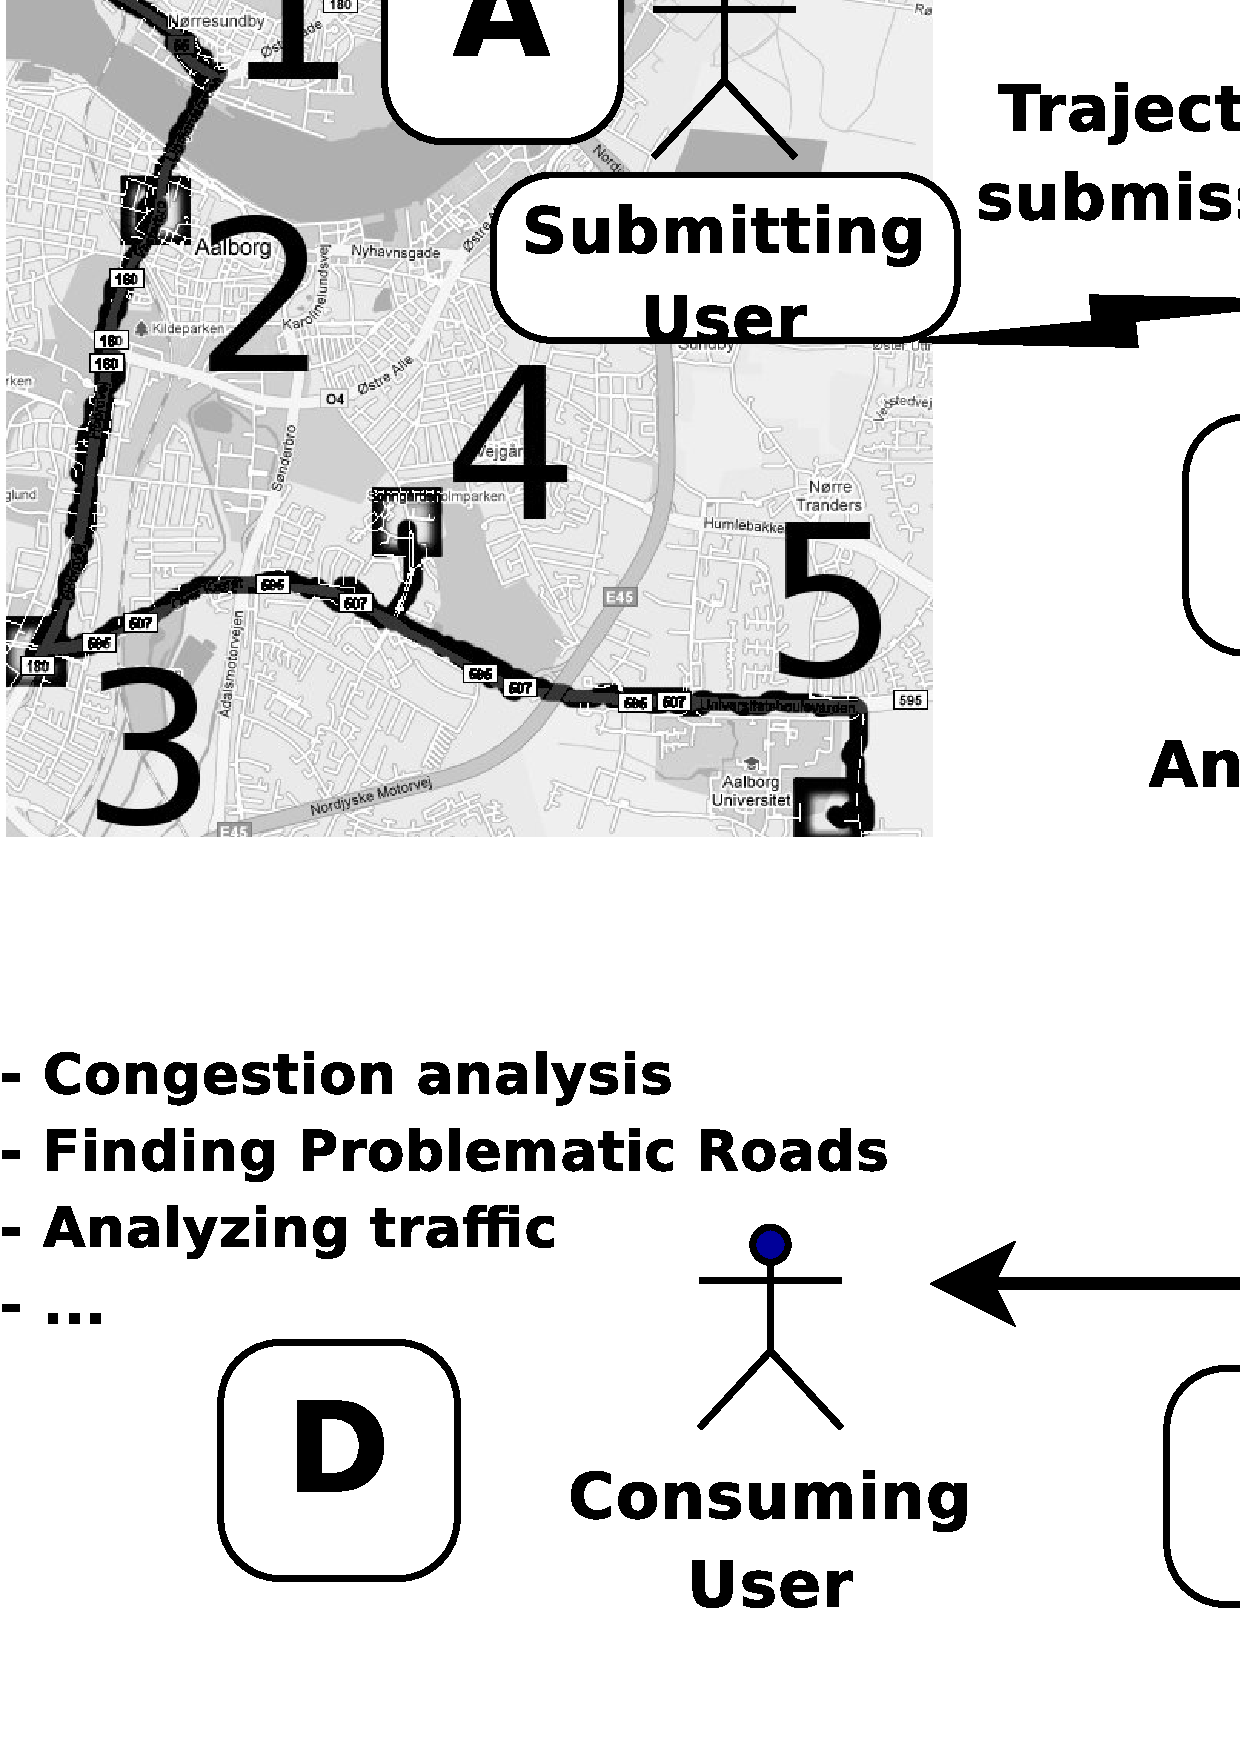
\includegraphics[page=1,scale=0.2]{images/overview.pdf}}
	\end{column}
	\begin{column}{0.5\textwidth}
		\begin{description}\itemsep 16pt
		\item[A] Privacy Aware User
		\item[B] Trusted Server
		\item[C] Public Untrusted Server
		\item[D] Service Providers
		\end{description}
	\end{column}
\end{columns}
\end{frame}%
\section{Baseline Competitors}

Intro to section; Why do we have baseline competitors, which ones will be introduced, and why those? 

LRU is a competitor, but can not achieve good performance because:
\begin{itemize}	
	\item Has no way to determine the usefulness of adding a path (i.e. no scoring function)
	\item Even if a path P is good (covers many queries), then if a sequence of consequtive queries comes which P can not cover, then it will be evicted.
	\item Has no way to optimize the number of paths in the cache, so available cache space may go unused.
	\item Querying the cache may require a scan of all paths in the cache
\end{itemize}

\section{Contribution} \label{sec:contribution}

Intro to section \\
Show benefits of a static cache over a dynamic cache.\\
List all advantages of a static cache solution \\
(\textit{Static cache} solves goal 2. has zero maintenance cost after filling the cache.)

explain what will be introduced, which sub-problems are considered, and which subsections presents what.


\subsection{Benefit model}
define benefit equations\\
Define optimization goal as a mathematical expfression to be minimized.

\subsection{Hardness Analysis}
Theoretical analysis showing how hard the problem is to solve for \spath caching.\\
show it is NP-Hard
 

\subsection{Greedy algorithm}
shows in more detail how we propose to solve our problem


\subsection{Statistics extration}

\subsubsection{Partition map} 
solves goal 1. reduce time on SP calc as it aids the cache with information on which paths may be useful.\\ 
discussion of kD-Tree.


\subsection{Cache representations and cache concepts} 

\subsubsection{Simple array of paths} - baseline for goal 2, unoptimized and expensive to use.

\subsubsection{Simple array of paths inverted list} - solves goal 2, reduces the query time of the cache.

\subsubsection{Graph representation} - solves goal 1, allows for more paths in cache, which should translate more cache hits.

\subsubsection{Sharing subpaths} - solves goal 1, allows for more paths in cache, translating to more cachehits. Unfortunally has a negative impact on goal 2 as it introduces some overhead in query time.

%
\subsection{Incremental update optimization}\label{sec:optIncUpd}

According the protocol when one (or more) location or vicinity enclosing
granule changes due to user movement, user's encrypted data must
be updated on the \ls by sending a $M_{el}$ message. Thus, in most
cases user's two consecutive $M_{el}$ messages would contain duplicated 
encrypted granules. 

The communication can be reduced by enabling so called \textit{incremental
updates}(\iuns). Here we introduce new type of message $M_{elUpd}$ that clients 
are allowed to send, instead of the $M_{el}$, when their locations change. 
It contains old items $u$, $l$, $g^*_l$ from $M_{el}$ and new items 
$\mathbf{g^*_{vDel}}$, $\mathbf{g^*_{vIns}}$, where $\mathbf{g^*_{vDel}}$, 
$\mathbf{g^*_{vIns}}$ define encrypted granules that must be deleted and inserted 
on the \ls in order to fully update some user $u$ encrypted data for level $l$. 
More precisely, if $m_1$ and $m_2$ are two consequent messages of type 
$M_{el}$ such that $m_1.u$=$m_2.u$ and $m_1.l = m_2.l$ then the
client may send a message $m_3$ of type $M_{elUpd}$ instead of $m_2$, where
$m_3.\mathbf{g^*_{vDel}}$ = $m_1.\mathbf{g^*_{v}}$
$\backslash$ $m_2.\mathbf{g^*_{v}}$ and $m_3.\mathbf{g^*_{vIns}}$ =
$m_2.\mathbf{g^*_{v}}$ $\backslash$ $m_1.\mathbf{g^*_{v}}$. 
Figure \ref{fig:ui_rf}a visualizes locations, vicinities, and 
vicinity-intersecting granules of user $u$ at two consequent 
time steps 0 and 1. Darkened sets of cells $\mathbf{g_{vDel}}$ and 
$\mathbf{g_{vIns}}$ visualize unencrypted representation of sets $g^*_{vDel}$ 
and $g^*_{vIns}$. Note, that introduction of $m_3$ helps reducing communication
only if $|m_3.\mathbf{g^*_{vDel}}|$ + $|m_3.\mathbf{g^*_{vIns}}|$ $<$
$|m_2.\mathbf{g^*_{v}}|$. 


Our presented client and server algorithms (See Alg. \ref{algCl}, \ref{algSrv})
can be easily modified to support incremental updates. In the current
implementation once a user goes from higher to lower levels (switches into
coarser granularity) granules of active level are being removed from stacks
on client and server ($GS$ and $GL$) without possibility to reuse them. The idea
is to preserve these granules on both client and server such that it would be
possible to update them utilizing $\mathbf{g_{vDel}}$, $\mathbf{g_{vIns}}$ or
$\mathbf{g^*_{vDel}}$, $\mathbf{g^*_{vIns}}$. 

The incremental updates impact on client communication is evaluated in 
Sec. \ref{sec:performStudy}.


\subsection{Grouping of Users}\label{subsec:grouping}

Currently all users in $\mathbf{M}$ share a single encryption function $\Psi$.
Security of $\Psi$ directly influence location privacy of all users in the
system. An adversary knowing $\Psi$ can easily decipher encrypted
granules of user current location and his vicinity. It is difficult to ensure
that the function $\Psi$ will stay secret in case of a high number of users
of the \vl service. Note that in case of leaked $\Psi$ users' minimum privacy 
requirements, specified by $L_{max}$, are still guaranteed, although it is 
desirable for users to obtain as much privacy as possible.

In order to limit affected users in case of leaked $\Psi$
\textit{grouping of users} can be enforced. Friend-grouping is
introduced in the long-paper version of the \ff \cite{ffinder}. The idea is
that all users in the system are grouped into possibly overlapping groups, so
that each user is put into one or more groups. Both friends and non-friends can
belong to the same group, but if two users are friends, they must be in at least
one common group. Each such group $G$ is assigned a distinct $\Psi_G$ function
and it is used by all members of $G$. Then if such $\Psi_G$ is leaked, only the
location privacy of the users in group $G$ are compromised.

Our presented algorithms of \vl can be easily modified to support friend
groups. The client and the server should treat each group individually such
that clients report their encrypted data for all groups that they are part of,
and the server independently analyzes encrypted data for every distinct group. 
In this paper, we do not consider how these groups are created. This can be done
automatically or manually by the users themselves.

%\input{articleFiles/rasterapproach.tex}
\section{Vulnerabilities \& Points of Attack}\label{sec:vulnerability}
We here address a few of the possible vulnerabilities
of the \vl approach. We assume correct behavior of both
the server and clients, and thus exclude attacks where an
attacker may want to modify either server or client to
e.g. trigger a ``spamming'' behavior.
The attackers goal will for each attack be to 
compromise the privacy of the largest possible number of
clients in the \vl system. 


\subsection{Compromised Client}\label{subsec:VulClient}
If an attacker gains control over a client
he will, for each group (see \ref{subsec:grouping})
the client is member of, have the $\Psi$ function 
used to calculate granules at the client.

If the client itself is compromised by an attacker, the $\Psi$ function
is not much help to him, since he cannot do much else than encode granules
sent to the server, but if one imagines that the attacker only temporarily
gains control, then he can use the $\Psi$ function to ``Clone'' the original
client. This problem is however easily made void by changing the $\Psi$ 
function regularly.

By using the \textit{battleship} method 
the attacker can guess the location of other users with same group 
membership as the compromised client\footnote{In the game of \textit{battleships} 
two opponents take turn to guess the location of the others battleships placed at 
secret locations in a grid.}.

One way an attacker may ``play battleship'' in order to find the location of
other users (with same group membership) would be to send a 
false vicinity covering the area he is interested in finding
other users, the attacker will then be notified by the server if any other 
user is within his false vicinity. The attacker then continues to cut the vicinity in half,
doing a binary search until he has found the granules of all users within the larger area
he initially sent his false vicinity for at the start\footnote{The amount of 
granules needed to be searched in the worst case is $\frac{c^{l+1}-1}{c-1}$ 
where $l$ is the number of levels needed to be traversed, and $c$ the number 
of granules each granule at level $l$ is divided into at $l+1$}.

By using groups this attack is already very limited, since each 
client is assumed to have far fewer friends then the overall amount
of users in the \vl system. Furthermore it is worth noticing that 
the attacker can never get an actual location of a user, since all he can get
a matching granule which corresponds to a spacial area and not a point.
There is also a build in limit on the amount of precision the attacker 
can achieve because each users $L_{max}$ is a limit on the precision that
any user will reveal. 
 
If we limit the attackers goal to only focus on a single friend, then 
using the binary search method described will enable the attacker to
track the single friend with the amount of vicinity splits he have to
do in worst case being: $\Theta(Log(\frac{B(cg)}{B(max)}))$ where $B(cg)$ is the
size of attackers current granule and $B(max)$ is the granule size at the maximum
precision attacker can get, either by setting his own $L_{max}$ or reaching the 
friends $L_{max}$.



\subsection{Compromised Server \& Client}\label{subsec:VulCliServ}
If the attacker has gained control over both the server and 
client, he has all info from \ref{subsec:VulClient} as well as 
all users encrypted center and vicinity granules, as well
as their group memberships (see \ref{subsec:grouping}).

The attacker can do the same as in \ref{subsec:VulClient}, 
only now the attacker can skip the \textit{battleship} step and decode
obfuscated location (center granules) of friends directly, making it
actually feasible to track all friends, this however is still
only valid for the groups that the compromised client is member of.

This attack has the same limitations as \ref{subsec:VulClient}, except
that since the attacker now skip the \textit{battleship} stage, it is 
feasible for the attacker to track many users (as long as they are in the
same group as the compromised client)
%
%\subsection{History}\label{subsec:VulHis} \ffh{not relevant, not risk}
%\textbf{info:} All users encrypted center and granules, 
%as well as their group memberships. The attacker collects data over time.
%
%\textbf{can do:} he can try to reason about how the center granule
%moves, by assuming it only moves a cell at a time,
%but this assumption does not hold so attacker can
%really reason about routes unless he has extra info
%about user (e.g. that user is from a specific region of a country,
%then he can maybe brute force possibilities in relation to road networks)


\subsection{Frequency}\label{subsec:VulFreq}
In this attack the server is compromised, and thus the
attacker knows all users encrypted center and granules, 
stored on the server, as well as their group memberships. 

The attacker can compare the frequency of users with same center and 
vicinity granules, the attacker can then see if many users
have the same granules, and reason about the actual location
(e.g. if attacker knows the national soccer team is playing, and he can
see many users suddenly all sharing granules).
The attacker can possibly collect the data over time and maybe make this attack
more efficient by looking for frequency in locations over time, e.g. if 
there is a central place most people must pass during the day (city center/a bridge etc.), 
the attacker can then use historical information to identify which granules 
correspond to this location.

There is a simple solution to thwart the effectiveness of this attack, and that is
to change the $\Psi$ function as some interval, making it impossible for the attacker
to compare granules from different intervals. If we furthermore assume that the server
would not be informed when $\Psi$ function is changed, then this attack becomes void.




\section{Experiments}\label{sec:experiments}
%
In this section, we evaluate the performance of our methods with our competitors on real datsets.
% We will conduct experiments
We have implemented two variants of our methods (SPC and SPC*).
%for extracting statistics of queries, benchmarking the cost of a shortest path call,
%and selecting promising paths from a query log $\mathcal{QL}$ into the cache.
They share the same techniques in Section~\ref{sec:BenefitDriven},
and only differ in their cache structures:
(i) SPC uses a path array cache (Section~\ref{sec:cacheLookup}), and (ii) SPC* uses the compressed graph cache (Sections~\ref{sec:cacheSubgraph},\ref{sec:cacheCompress}).
%
Our competitors are LRU (a dynamic caching method) and HQF (a static caching method).
They have been introduced in Section~\ref{sec:competitors}.
All the above methods are written in C++.
We conduct our experiments on an Intel i7 3.4GHz PC running Debian.

%  (ii) SPC$^+$ uses a graph cache (Section~\ref{sec:cacheSubgraph}),
%SPC, our method, with the 3 cache representation schemes - List cache, Graph cache, Compressed Graph cache - described in section

We will evaluate the above methods for a cache located at the proxy, and for a cache located at the server.
For the proxy scenario, the performance measure is the hit ratio.
For the server scenario, the performance measures are: (i) the total running time of the server,
and (ii) the total number of road network nodes visited.


%in both the proxy
%well both when considering the Proxy and Server scenario

%To compare how well we have done, we have implemented two baseline competitors, LRU and HQF. LRU is a dynamic caching method which evicts the Least recently used cache item if there is no space in the cache for new entries. HQF adds to the cache, the \spaths from the most frequent start-/end-points in the training data.





%Aalborg: total nodes in SPs from training set: 352032 in 1643 paths

%Beijing: total nodes in SPs from training set: 316400 in 6479 paths



%This is the most common usage of static caching in the web caching literature \cite{BaezaYates07}.


% In this section, we present the results of performance
% experiments, demonstrating the efficiency and realworld applicability of the proposed algorithms. We


\subsection{Experimental Setting}
%
We are unable to obtain real query log from online shortest path services (e.g., Google Map), due to their privacy policies.
Thus, we can only simulate a query log from a trajectory dataset.
For each trajectory, we extract its start location and its end location as the
source $v_s$ and destination $v_t$ of a shortest path query respectively.

We have used two real datasets and their details can be found in Table~\ref{tab:datasetsize}.
Each dataset consists of (i) a collection of trajectories (which can be used to simulate a query log), and 
(ii) a corresponding road network for the trajectories.

%Which historical query datasets do we have, and what is their size and origin.

%- Aalborg: Query workload from and around the Danish city of Aalborg

%- Beijing: Query workload from Beijing



Following the experimental methodology of static caching~\cite{Ozcan2011},
we divide the query log into two equal sets.
The {\em historical query log} set is used for defining query frequencies and
for filling the cache content.
The {\em query workload set} set can only used for testing the performance of our method.


%We do not give a default size for the query-datasets Maps, as we will execute all of our tests, described in section \ref{subsec:expProxy} and \ref{subsec:expServer}, for each dataset.


\begin{table}
\center
\begin{tabular}{|c|r|r|r|}\hline
Dataset & $\#$ Trajectories / Queries & $\#$ Nodes & $\#$ Edges \\\hline
Aalborg & 4.401  & 129.680 & 137.470 \\\hline
Beijing & 12.928 & 76.226 & 85.882 \\\hline
\end{tabular}
\caption{Description of real datasets}
\label{tab:datasetsize}
\end{table}
%% Aalborg = Aalborg
%% Beijing = Beijing


%GPS trajectories

%according to XXX l

%The size of training and test query datasets are given already. The size of each dataset, as well as the map they are captured on, is given in table \ref{tab:datasetsize}.



%% Aalborg = Aalborg
%% Beijing = Beijing


%We do not give a default size for the query-datasets Maps, as we will execute all of our tests, described in section \ref{subsec:expProxy} and \ref{subsec:expServer}, for each dataset.




All caching methods, SPC, SPC*, HQF, and LRU, share a number of common settings which, unless stated otherwise, will be set to their default values:
The number of levels in the kD-tree is 14 (i.e. 16,384 regions). We will use the list cache representation as the default cache representation, where each vertex use one byte. The default cache size is set to 625 kB.


The default cache size, as well as the maximum cache size in later experiments (Fig.~\ref{fig:cSizeVsHitRatio}, \ref{fig:cacheSizeVsHitRuntime}, \ref{fig:cacheSizeVsNodesvisited}), is choosen baring in mind the size of the Aalborg and Beijing query logs. 
Had we had access to large datasets of real query logs, from online shortest path serveice providers, we would use a large cache size like 1 GB.

% 
% 
% The size of our datasets is the limiting factor
% 



\label{fig:cacheSizeVsHitRuntime}

\label{fig:cacheSizeVsNodesvisited}


% - Which parameters are common for all tests
% - What are the ranges/values each parameter can take.
% - Which parameters are set to a default value unless otherwise stated (and what are the default values)
% - Which methods, and in which configuration, do we consider.



\subsection{Caching in the Proxy Scenario}\label{subsec:expProxy}
%
In the proxy scenario, the shortest path call API would issue a shortest path query to the server,
rather than performing computation by itself (see Section~\ref{sec:benchmark}).
Since the total cost is dominated by the communication round-trip time with server,
we use the cache hit ratio as the performance measure in this scenario.

For both datasets we vary the cache size and kD-tree levels to show the impact on the cache hit ratio. We have implemented a number of optimizations to the cache storage (See sec. \ref{sec:CacheStruct}) and show their impact on the cache hit ratio.


\stitle{Effect of the cache size}
%
In Figure~\ref{fig:cSizeVsHitRatio}, we measure the hit ratio of the methods
while varying the cache size from 1 kB to 5 MB.


\begin{figure}[htb]
\center
  \begin{tabular}{@{}c@{ }c@{}}
     \includegraphics[width=0.5\columnwidth]{figures/cachesize_hitratio_aal.pdf}
     &
     \includegraphics[width=0.5\columnwidth]{figures/cachesize_hitratio_bei.pdf}
      \\
     (a) Aalborg & (b)  Beijing
     \end{tabular}
\caption{Hit ratio vs. cache size }
\label{fig:cSizeVsHitRatio}
\end{figure}

% \begin{itemize}
% \item We can see SPC* performs much better than competitors
% \item LRU perform well on small cache sizes, but the cache hit ratio quickly level out and stop growing, thus LRU is not scalable.
% \item HQF performance is very consistent, with the hit ratio varying only slightly. The hit ratio does however stay at just over 1\% for Aalborg experiments and around 0.2\% for Beijing experiments. It is not usable
% \item We observe that SPC initially does not grow as fast as LRU, but the growth continues as we increase cache size, unlike for LRU.
% \item SPC* grows faster than LRU and gets better cache hit ratio at all cache sizes than LRU and SPC, except for the smallest cache size.
% \item The test on the Aalborg vs. Beijing sets show that SPC performs much better on the Aalborg set, where as LRU performs about 50\% worse. This can be explained by the fact that both methods rely on users behaving consistently over time, but where SPC relies on global consistency in user behavior, LRU need local consistency too. This makes SPC/SPC* more robust and we can expect them to always outperform LRU.
% \end{itemize}
{\color{red}
We can see that LRU consistently perform worse than SPC and SPC$^*$ for all cache sizes. The cache hit ratio stabilizes at about 26 and 40\% for Aalborg and Beijing respectively. Since LRU levels out at a much lower cache hit ratio than all of it's competitors it is not a suitable choice for \spath cacheing.


The performance of HQF is quite low at smaller cache sizes, 

The performance of HQF is very consistent, with the hit ratio varying only slightly. The hit ratio stays at just over 1\% for Aalborg experiments and around 0.2\% for Beijing experiments. The low hit ratio makes it not scalable and unusable for \spath caching.
}

SPC does not grow as fast as LRU for smaller cache sizes, but while the growth of LRU quickly stabilizes then SPC continues to grow and outperforms both LRU and HQF.
SPC* outperforms both LRU and SPC by a large margin, only shortly having a lower cache hit ratio at smaller cache sizes. The test on Aalborg vs. Beijing  show that SPC performs much better on the Aalborg set, where as LRU performs about 50\% worse. This can be explained by the fact that both methods rely on users behaving consistently over time, but where SPC relies on global consistency in user behavior, LRU need local consistency too. This makes SPC/SPC* more robust and we expect them to always outperform LRU.



\stitle{Effect of the kD-tree level}
%
In Figure~\ref{fig:levelVsHitRatio}, we vary the kD-tree level from 8 to 18 levels and show that using a kD-tree of about 14 levels can significantly increase the cache hit ratio of both the Aalborg and Beijing dataset. SPC* performs better than SPC.


\begin{figure}[htb]
\center
  \begin{tabular}{@{}c@{ }c@{}}
     \includegraphics[width=0.5\columnwidth]{figures/split_hitratio_aal.pdf}
     &
     \includegraphics[width=0.5\columnwidth]{figures/split_hitratio_bei.pdf}
      \\
     (a) Aalborg & (b)  Beijing
     \end{tabular}
\caption{Hit ratio vs. Levels}
\label{fig:levelVsHitRatio}
\end{figure}

On both dataset SPC* outperforms SPC by a large margin. On the city X dataset SPC* achieves more than a 50\% increase in hit ratio, and when compared to SPC, it achieves a relative performance gain of 500-900\% at low levels up to the peak performance at level 14.
On the Y dataset SPC* gets a lower hit ratio, but it still achieves more than 50\% cache hit ratio. The results are still very impressive, with SPC* performing 200-400\% better than SPC at all levels.

% \noindent
% \begin{tabular}{|l |p{0.58\columnwidth} |l |}
% \hline
% \textbf{Parameter} & \textbf{Meaning / used for} & \textbf{Standard value} \\\hline
% Mapfile & The map which the test is performed on & \\\hline
% NumQueries & Number of \spath queries in test & \\\hline
% QuerySet & which dataset is used to provide queries & \\\hline
% TrainSet & For generating region statistics, which dataset is used & \\\hline
% CacheSize & Size of cache in bits & \\\hline
% cacheType & Type of cache representation (list/graph) & \\\hline
% kD-tree & Hight of the kD-tree & \\\hline
% avgLenght & Average length of a shortest path & \\\hline
% \end{tabular}

% Write experiments to examine performance of goal 1 \& 2
% Test ideas (several ideas may be combined, like item 1 can be done on all datasets from item 2):\\
% \begin{itemize}
% \item increase kd-tree hight from 0-18
% \item different maps [Oldenburg, Aalborg, Beijing]
% \item compare cache type performance
% \item compare with baseline methods. [LRU dynamic, Dynamic(maxLevel)]
% \item vary the cache size [10.000-2560000]
% \item vary number of queries. [only for synthetic data]
% \end{itemize}

\subsection{Caching in the Server Scenario}\label{subsec:expServer}
%
In the server scenario, the shortest path API has to invoke a shortest path algorithm.
Thus, the running time is the most important performance measure. We also measure the number of nodes visited in a shortest path algorithm, which serves an indicator of the running time.
%On a server our aim is slightly different than on the Proxy, as we also have to consider that there may be some paths that are so small that it may be cheaper to simply re-calculate the result, instead of caching it.
%For the server scenario we will test the cache hit ratio, running time, and Nodes visited.
%For all three experiments
%We will vary kD-tree levels and cache size in the following experiments.
As a case study, we use the Dijkstra's algorithm as the shortest path algorithm.

In the following experiments, the running time (and nodes visited) refer to the total running time (and nodes visited) for processing the entire query workload. The running time is measured in the unit of seconds.





\stitle{Estimation of shortest path running cost}
%
First, we test the estimation error of our cost estimation technique proposed in Section~\ref{sec:benchmark}.
We measure the error percentage in terms of the relative error between the actual cost and the estimated cost.
Table~\ref{tbl:estcost} shows the estimation error of our technique
as a function of: (a) the number of landmark $|U|$, and (b) the size of the samples $S$.
The default values are: $|U|=20$ and $S=100$.
The majority of errors are below 30\% and thus our estimation technique is reasonably accurate.


%% Aalborg: average cost = 136347/2 = 68173
%%  Beijing: average cost = 79603/2 = 39801
%  average because random node chosen



\begin{table}
\center
\begin{tabular}{cc}
    \begin{tabular}{|c|c|c|}
    \hline
    $|U|$ & Aalborg & Beijing \\ \hline \hline
     5 & 35.5 & 33.3 \\ \hline
     10 & 25.4 & 28.2 \\ \hline
     20 & 22.2 & 23.9 \\ \hline
     40 & 19.4 & 23.0  \\ \hline
     80 & 19.9 & 21.9 \\ \hline
    \end{tabular}
    &
    \begin{tabular}{|c|c|c|}
    \hline
    $S$ & Aalborg & Beijing \\ \hline \hline
     25 & 23.4 & 28.8 \\ \hline
     50 & 20.7 & 28.4 \\ \hline
     100 & 22.2 & 23.9 \\ \hline
     200 & 20.4 & 22.7 \\ \hline
     400 & 21.1 & 21.3 \\ \hline
    \end{tabular}
    \\
    (a) varying number of landmark $|U|$ & (b) varying sample size $S$
\end{tabular}
    \caption{Average error percentage of cost estimation}
    \label{tbl:estcost}
\end{table}








%
\stitle{Effect of the kD-tree level}
%
In Figure~\ref{fig:levelVsHitRatio}, we again vary the kD-tree level from 8 to 18 levels. All three experiments shows a consistent advantage of using SPC* over SPC. SPC* still has an even higher advantage than in the proxy scenario, performing around 950\% better than SPC at its best. SPC, however, has a very low hit ratio in the server scenario, on both the city X and Y datasets. In figure \ref{fig:levelVsruntime}a and b we can see that SPC* is very fast at answering the query workload. SPC has a quite stable time in both figure\ref{fig:levelVsruntime}a and b, while the time for SPC* to answer the query workload actually decreases with more regions. In figure \ref{fig:levelVsNodesvisited} we can see that SPC* visits far fewer nodes than SPC, during shortest path calculations. This is expected since SPC* can answer many more queries from its cache.




\begin{figure}[htb]
\center
  \begin{tabular}{@{}c@{ }c@{}}
     \includegraphics[width=0.5\columnwidth]{figures/split_hitratio_aal_server.pdf}
     &
     \includegraphics[width=0.5\columnwidth]{figures/split_hitratio_bei_server.pdf}
      \\
     (a) Aalborg & (b)  Beijing
     \end{tabular}
\caption{Hit ratio vs. Levels}
\label{fig:levelVsHitRatio}
\end{figure}

\begin{figure}[htb]
\center
  \begin{tabular}{@{}c@{ }c@{}}
     \includegraphics[width=0.5\columnwidth]{figures/split_runtime_aal_server.pdf}
     &
     \includegraphics[width=0.5\columnwidth]{figures/split_runtime_bei_server.pdf}
      \\
     (a) Aalborg & (b)  Beijing
     \end{tabular}
\caption{Runtime vs. Levels}
\label{fig:levelVsruntime}
\end{figure}

\begin{figure}[htb]
\center
  \begin{tabular}{@{}c@{ }c@{}}
     \includegraphics[width=0.5\columnwidth]{figures/split_nodes_aal_server.pdf}
     &
     \includegraphics[width=0.5\columnwidth]{figures/split_nodes_bei_server.pdf}
      \\
     (a) Aalborg & (b)  Beijing
     \end{tabular}
\caption{Nodes Visited vs. Levels}
\label{fig:levelVsNodesvisited}
\end{figure}






\stitle{Effect of the cache size}
%
In the following experiments, we vary the cache size and observe the effect on the running time and nodes visited during shortest path calculations.






\begin{figure}[htb]
\center
  \begin{tabular}{@{}c@{ }c@{}}
     \includegraphics[width=0.5\columnwidth]{figures/cachesize_runtime_aal.pdf}
     &
     \includegraphics[width=0.5\columnwidth]{figures/cachesize_runtime_bei.pdf}
      \\
     (a) Aalborg & (b)  Beijing
     \end{tabular}
\caption{Runtime vs. Cache Size}
\label{fig:cacheSizeVsHitRuntime}
\end{figure}

In Figure \ref{fig:cacheSizeVsHitRuntime} and \ref{fig:cacheSizeVsNodesvisited}, for both the city X and Y dataset,  we can see that the graph looks similar to Figure \ref{fig:cSizeVsHitRatio}, but in the upside-down manner. This is to be expected, since a higher cache hit ratio gives fewer \spath calculations, and a lower runnig time when answering queries.

\begin{figure}[htb]
\center
  \begin{tabular}{@{}c@{ }c@{}}
     \includegraphics[width=0.5\columnwidth]{figures/cachesize_nodes_aal.pdf}
     &
     \includegraphics[width=0.5\columnwidth]{figures/cachesize_nodes_bei.pdf}
      \\
     (a) Aalborg & (b)  Beijing
     \end{tabular}
\caption{Nodes Visited vs. Cache Size}
\label{fig:cacheSizeVsNodesvisited}
\end{figure}

%\section{Future work} \label{sec:future}
Lorem ipsum dolor sit amet, consectetur adipiscing elit. Pellentesque elementum elementum turpis. Pellentesque diam elit, scelerisque eget, mollis vel, aliquet feugiat, dolor. Nunc dignissim tristique risus. Maecenas molestie tellus sit amet neque. Etiam porttitor posuere lacus. Etiam mi diam, dapibus hendrerit, condimentum in, malesuada eget, libero. Aliquam enim. Nam dolor dolor, fermentum et, faucibus sodales, iaculis sed, justo. Integer sagittis placerat justo. Cum sociis natoque penatibus et magnis dis parturient montes, nascetur ridiculus mus. Donec ullamcorper metus at turpis. Proin vel risus. Nam libero lectus, gravida vel, aliquet a, vestibulum a, lorem. Mauris eget quam non enim placerat consequat. Nam dolor lacus, lacinia et, posuere vitae, sollicitudin vel, eros.
\section{Conclusion}
\subsection{Conclusion} % Bookmark information, displayed in the progress tree
\begin{frame}[red] %hmm.. thought i could change colour here :S
\frametitle{Conclusion}

\begin{itemize}
	\item Novel Privacy Profile to specify spatial-temporal sensitivity of a POI.
	\item Introduced t-anonymity
	\item Introduced Protection types and schemes.

\end{itemize}

 
\end{frame}

\subsection{Future Work} % Bookmark information, displayed in the progress tree
\begin{frame}[red] %hmm.. thought i could change colour here :S
\frametitle{Future Work}

\begin{itemize}
	\item Algorithm
	\item Performance study

\end{itemize}
\end{frame}


\begin{frame}[red] %hmm.. thought i could change colour here :S
\frametitle{End of Presentation}

\vspace{20mm}
\begin{center}
    \Huge Thank You For Listening
\end{center}

\end{frame}


%-------------------------------------------------------------------------

\bibliographystyle{splncs}

\bibliography{bibliography}

\end{document}